% Intended LaTeX compiler: pdflatex
\documentclass[10pt,letterpaper]{article}

\usepackage[utf8]{inputenc}
\usepackage[T1]{fontenc}
\usepackage{graphicx}
\usepackage{longtable}
\usepackage{wrapfig}
\usepackage{rotating}
\usepackage[normalem]{ulem}
\usepackage{amsmath}
\usepackage{amssymb}
\usepackage{capt-of}
\usepackage{hyperref}
\usepackage[utf8]{inputenc}
\usepackage{xifthen}
\usepackage[T1]{fontenc}
\renewcommand*\familydefault{\sfdefault}
\usepackage{moresize}
\usepackage[letterpaper]{geometry}
\geometry{top=1.00cm, bottom=0.0cm, left=1.0cm, right=1.0cm}
\usepackage{fancyhdr}
\pagestyle{fancy}
\setlength{\headheight}{-15pt}
\usepackage[none]{hyphenat}
\setlength{\parindent}{0mm}
%-----------------------------------------------------------------------------------------------------------------------------------------------%
%	The MIT License (MIT)
%
%	Copyright (c) 2015 Jan Küster
%
%	Permission is hereby granted, free of charge, to any person obtaining a copy
%	of this software and associated documentation files (the "Software"), to deal
%	in the Software without restriction, including without limitation the rights
%	to use, copy, modify, merge, publish, distribute, sublicense, and/or sell
%	copies of the Software, and to permit persons to whom the Software is
%	furnished to do so, subject to the following conditions:
%
%	THE SOFTWARE IS PROVIDED "AS IS", WITHOUT WARRANTY OF ANY KIND, EXPRESS OR
%	IMPLIED, INCLUDING BUT NOT LIMITED TO THE WARRANTIES OF MERCHANTABILITY,
%	FITNESS FOR A PARTICULAR PURPOSE AND NONINFRINGEMENT. IN NO EVENT SHALL THE
%	AUTHORS OR COPYRIGHT HOLDERS BE LIABLE FOR ANY CLAIM, DAMAGES OR OTHER
%	LIABILITY, WHETHER IN AN ACTION OF CONTRACT, TORT OR OTHERWISE, ARISING FROM,
%	OUT OF OR IN CONNECTION WITH THE SOFTWARE OR THE USE OR OTHER DEALINGS IN
%	THE SOFTWARE.
%
%
%-----------------------------------------------------------------------------------------------------------------------------------------------%

\lhead{}
\chead{
  \textcolor{txtcol}{\textbf{Consultant and Software Engineer}} \textcolor{sectcol}{$\oplus$}
  \textcolor{txtcol}{\textbf{Roanoke, Virgina}} \textcolor{sectcol}{$\oplus$}
  \textcolor{txtcol}{\textbf{davidconner@xel.io}} \textcolor{sectcol}{$\oplus$}
  \textcolor{txtcol}{\textbf{+1 (540) 761-1257}}
}
\rhead{}

%	TABLE /ARRAY/LIST DEFINITIONS

% this seems to think that it's beginning a document

% \newcolumntype{x}[1]{%
% >{\raggedleft\hspace{0pt}}p{#1}}%

%	GRAPHICS DEFINITIONS

\usepackage{graphicx}

%\floatstyle{boxed}
%\restylefloat{figure}

%============================================================================%
%	DEFINITIONS
%============================================================================%

% 	HEADER

% remove top header line
\renewcommand{\headrulewidth}{0pt}

%remove botttom header line
\renewcommand{\footrulewidth}{0pt}

%remove pagenum
\renewcommand{\thepage}{}

%remove section num
\renewcommand{\thesection}{}

% 	ARROW GRAPHICS in Tikz

% a six pointed arrow pointing to the right
\newcommand{\tzrarrow}{ (0,0.2) -- (0.1,0) -- (0.3,0) -- (0.2,0.2) -- (0.3,0.4)
  -- (0.1,0.4) -- cycle;}

% a six pointed arrow poiting to the left
\newcommand{\tzlarrow}{(0,0) -- (0.2,0) -- (0.3,0.2) -- (0.2,0.4) -- (0,0.4) -- (0.1,0.2) -- cycle;}

% include the left arrow into a tikz picture
% param1: fill color
%
\newcommand{\larrow}[1]
{\begin{tikzpicture}[scale=0.58]
	 \filldraw[fill=#1!100,draw=#1!100!black]  \tzlarrow
 \end{tikzpicture}
}

% include the right arrow into a tikz picture
% param1: fill color
%
\newcommand{\rarrow}
{
\begin{tikzpicture}[scale=0.7]
	\filldraw[fill=sectcol!100,draw=sectcol!100!black] \tzrarrow
 \end{tikzpicture}
}

%	custom sections


% create a coloured box with arrow and title as cv section headline
% param 1: section title
%
\newcommand{\cvsection}[1]{
\colorbox{bgcol}{\makebox[1\linewidth][l]{
	\larrow{sectcol} \hspace{-8pt} \larrow{sectcol} \hspace{-8pt} \larrow{sectcol} \textcolor{txtcol}{\textbf{#1}}\hspace{4pt}
}}
}

\newcommand{\cvbar}{
  \hfill\textcolor{softcol}{\rule{3cm}{.6}}\hfill
}

  % \hfill\textcolor{symcol}\hspace{0.1cm}o\hspace{0.2cm} o \hspace{0.4cm} o \hspace{0.8cm} o \hspace{16cm}\hfill
  
% \hfill \colorbox{symcol}{\makebox[0.1\linewidth][c]{ #1 } } \hfill


%create a coloured arrow with title as cv meta section section
% param 1: meta section title
%
\newcommand{\metasection}[2]{
	\begin{tabular*}{0.9\linewidth}{p{0.15\linewidth} p{0.70\linewidth}}
      \hfill\normalsize{\textbf{\textcolor{sectcol}{#1}}}&\textcolor{txtcol}{#2}\\
	\end{tabular*}
}

%	 CV EVENT

% creates a stretched box as cv entry headline followed by two paragraphs about
% the work you did
% param 1:	event time i.e. 2014 or 2011-2014 etc.
% param 2:	event name (what did you do?)
% param 3:	institution (where did you work / study)
% param 4:	what was your position
% param 5:	some words about your contributions
%
% \newcommand{\cvevent}[4] {
%   \begin{flushleft}\\[-5pt]
%     \begin{tabular*}{0.9\linewidth}{l c r}
%       #3 & #2 & \parbox{0.20\linewidth}{\raggedright #1}
%     \end{tabular*}
%     \vspace{\spread}
%     \begin{tabular*}{1\linewidth}{p{0.001\linewidth} p{0.9\linewidth}}
%       #4
%     \end{tabular*}
%   \end{flushleft}
% }

\newcommand{\cvexp}[4] {
  \begin{flushleft}\\[-16pt]
    \vspace{\spread}
    \textbf{\textcolor{txtcol}{#4}}\hfill\textit{#2}\hfill\scriptsize{#3}\hfill\small{\textbf{#1}}\\[-5pt]
  \end{flushleft}
}

\newcommand{\cvexprecent}[5] {
  \begin{flushleft}\\[-5pt]
    \textbf{\textcolor{txtcol}{#4}}\hfill\textit{#2}\hfill\scriptsize{#3}\hfill\small{\textbf{#1}}\\[-5pt]
    \vspace{\spread}
    \begin{tabular*}{1\linewidth}{p{0.001\linewidth} p{0.9\linewidth}}
      #5
    \end{tabular*}
  \end{flushleft}
}

\newcommand{\cvevent}[4] {
  \begin{flushleft}\\[-5pt]
    \textbf{\textcolor{txtcol}{#3}}\hfill\textit{#2}\hfill\small{\textbf{#1}}\\[-5pt]
    \vspace{\spread}
    \begin{tabular*}{1\linewidth}{p{0.001\linewidth} p{0.9\linewidth}}
      #4
    \end{tabular*}
  \end{flushleft}
}

\newcommand{\cvpoint}[1] {
	\larrow{bgcol} & #1
}

\newcommand{\cvrule}[2] {
\vspace{#1}
  \hfill\textcolor{softcol}{\rule{8cm}{.4}}\hfill
\vspace{#2}
}

% creates a stretched box as
\newcommand{\cveventmeta}[2] {
	\mbox{\mystrut \hspace{87pt}\textit{#1}}\\
	#2
}

% CUSTOM STRUT FOR EMPTY BOXES
%----------------------------------------- -----------------------------------------------
\newcommand{\mystrut}{\rule[-.3\baselineskip]{0pt}{\baselineskip}}

% CUSTOM LOREM IPSUM

\newcommand{\lorem}
{Lorem ipsum dolor sit amet, consectetur adipiscing elit. Donec a diam lectus.}

% SPREAD

\newcommand{\spread}{7pt}



\usepackage{multicol}
\usepackage{multirow}
\usepackage{array}
\usepackage{enumitem}
\usepackage{graphicx}
\usepackage{wrapfig}
\usepackage{float}
\usepackage{tikz}
\usepackage{tikz-3dplot}
\usepackage{tcolorbox}
\tcbuselibrary{most}
\usetikzlibrary{shapes, backgrounds, mindmap, trees, math}
\usepackage{color}
\definecolor{bgcol}{RGB}{140,130,120}
\definecolor{sectcol}{RGB}{30,25,18}
\definecolor{softcol}{RGB}{195,205,175}
\definecolor{txtcol}{RGB}{25,20,15}
\definecolor{softcol2}{RGB}{175,195,145}
\date{}
\title{David Conner Resume (twocol, letter)}
\hypersetup{
 pdfauthor={},
 pdftitle={},
 pdfkeywords={},
 pdfsubject={},
 pdfcreator={},
 pdflang={English}}
\usepackage{biblatex}

\begin{document}

\pagestyle{fancy}
\begin{minipage}[t]{0.490\textwidth}
\vspace{\spread} 
\label{sec:org383cb50}

%	TITLE HEADLINE
\hspace{-0.25\linewidth}\colorbox{bgcol}{\makebox[1.25\linewidth][c]{\textcolor{bgcol}{\rule[-1mm]{1mm}{1.0cm}} \HUGE{\textcolor{txtcol}{\textsc{David Conner}}}}}
%---------------------------------------------------------------------------------------
%	HEADER IMAGE
% \hspace{-0.25\linewidth}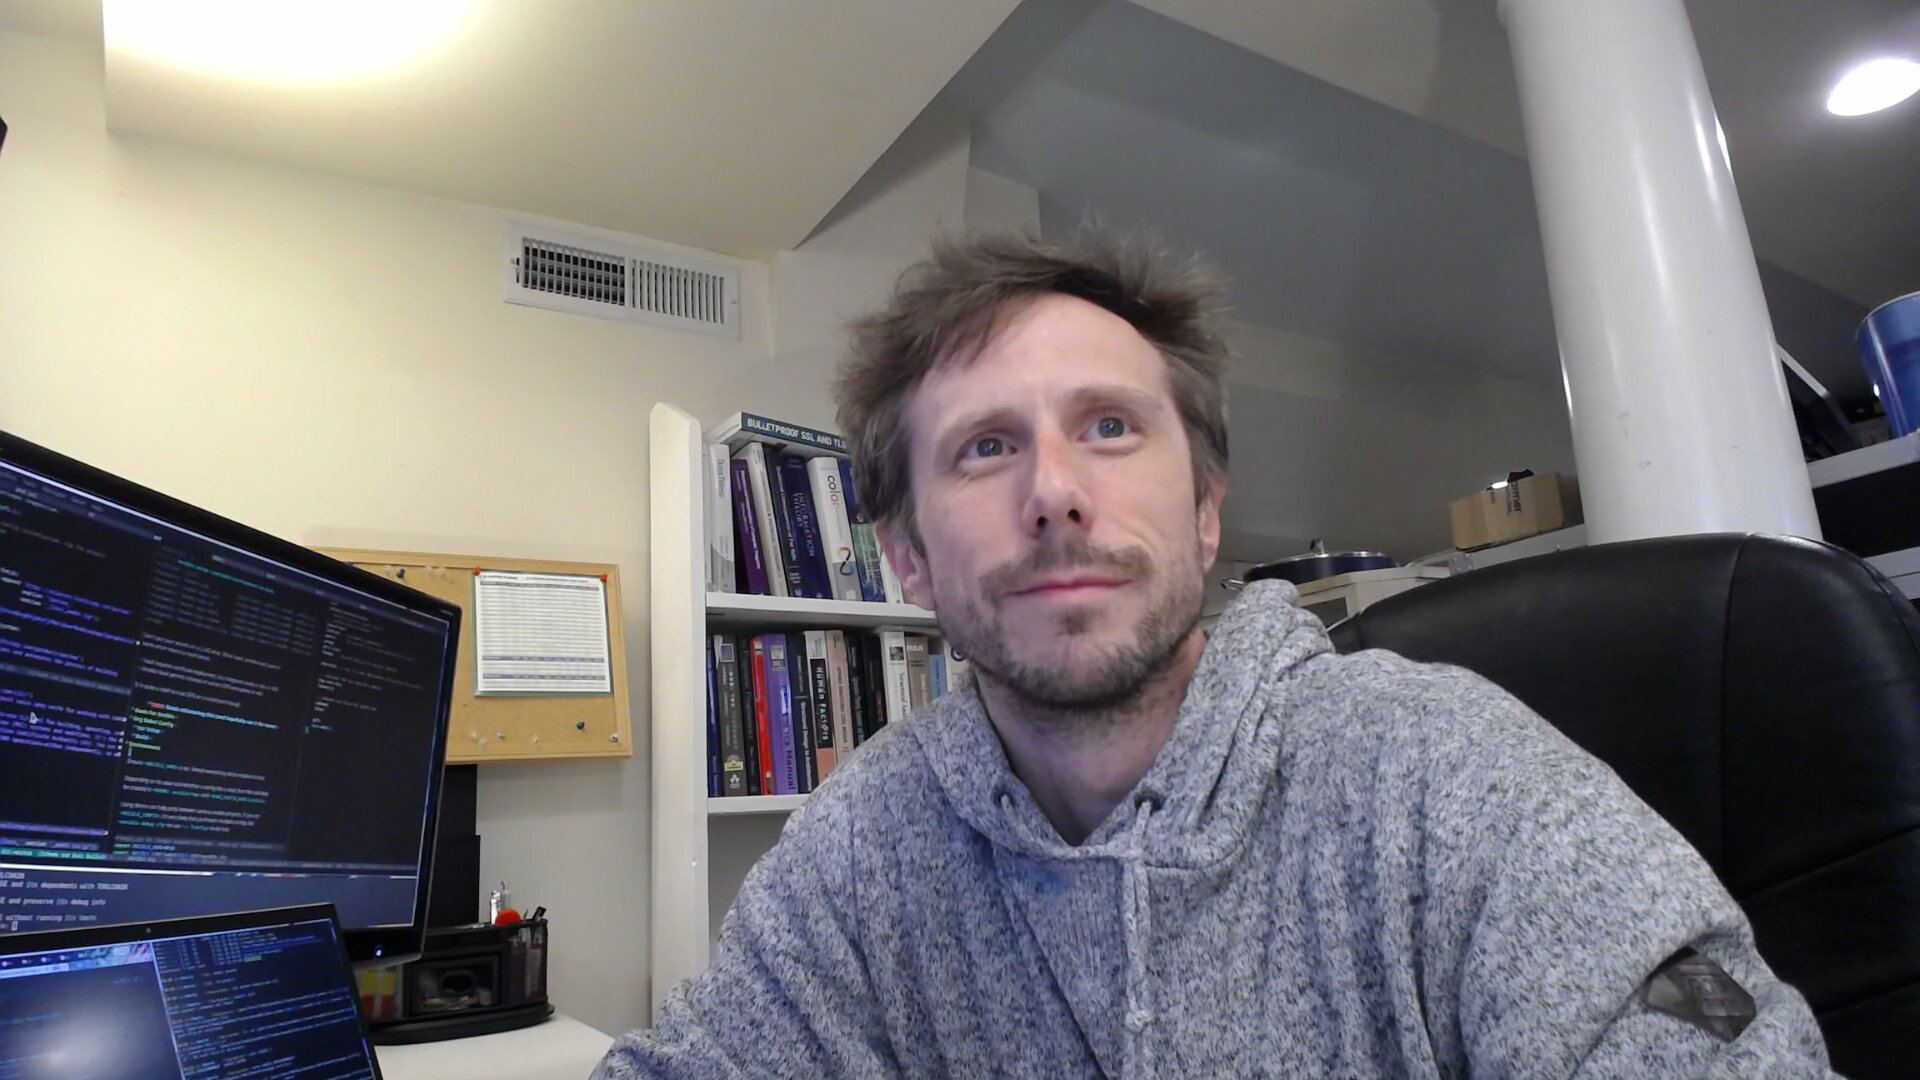
\includegraphics[width=1.2725\linewidth]{myphoto.jpg} %use full size
%---------------------------------------------------------------------------------------
%	QR CODE (optional)
%\vspace{-100pt}
%\hspace{0.59\linewidth}
%
\includegraphics[width=88pt]{qrcode}
%\normalsize
% \pareindent here is a hack
\setlength{\parindent}{5mm}

\vspace{-0.1cm}\\
\small{Software engineer with experience in networking, databases, containers,
and web applications. Seeking role that leverages software to solve domain-specific
problems, whether as an application programmer or devops. Experience integrating
disparate systems with minimal service interruptions and no loss of data.}

\small{Fast learner with a thirst for staying ahead in technology world.
Prefers the source code as the canonical documentation for most tools, but
also reads the docs.}\\[4pt]

\end{minipage}
\hfill
\begin{minipage}[t]{0.490\textwidth}
\vspace{\spread} 
\label{sec:org10db588}

\cvsection{Skills \& Tools}
\metasection{Linux}{Docker, Podman, Systemd, RPM, Guix, NixOS, LVM, Qemu, KVM}
\metasection{Security}{Firewalls, GPG, PIV, Yubikey, X.509, SOPS, AGE, Crypto}
\metasection{Homelab}{Cisco, VyOS, VLANs, NAT, Bare Metal, Proxmox}
\metasection{Cloud}{Terraform, k8s, GCP, DNS}
\metasection{Lang}{Ruby, Python, Java, JS, TS, Clojure, Scheme, Julia, Swift, Lua}
\metasection{Tools}{Bash, Ansible, Emacs, SSH \& Tunnels, Tmux, Make, Git \& Worktrees, Jupyter, AMD ROCm}
\metasection{HW}{Robotics, VTY Console, GNU Screen}
\metasection{Data}{Reporting, ETL, jq, JSON \& Schemas, Postgres, MSSQL, SQLite3, Parquet, graphviz}
% \cvrule{-6pt}{0pt}

\end{minipage}
\hfill
\begin{minipage}[t]{0.490\textwidth}
\vspace{\spread} 
\label{sec:orge2db43f}

\vspace{2pt}
%---------------------------------------------------------------------------------------
%	NON-PROFIT
\cvsection{Non-Profit}
\cvevent{2025-2026}{Programming Mentor}{Star City Robotics}
{\cvpoint{Maintained Ender-3 Pro and Raise3D printers. Synced Ender-3 configurations for PLA plastics}\\ % \\[2pt]
\cvpoint{Created an Autodesk Fusion CNC config for a Velocity CNC}\\ % \\[2pt]
\cvpoint{Collected notes on almost all equipment including support links and digital copies of manuals}} \\[\spread]
%
\cvrule{-6pt}{0pt}
%
\cvevent{2025-2026}{Programming Mentor}{Star City Robotics}
{\cvpoint{Maintained Ender-3 Pro and Raise3D printers. Synced Ender-3 configurations for PLA plastics}\\ % \\[2pt]
\cvpoint{Created an Autodesk Fusion CNC config for a Velocity CNC}} \\[\spread]
%
%---------------------------------------------------------------------------------------
%	EXPERIENCE
\cvsection{Experience}
\cvexprecent{2022-2023}
{Eng. Student Aide}
{Roanoke, VA}
{Virginia Western}
{\cvpoint{Maintained Ender-3 Pro and Raise3D printers. Synced Ender-3 configurations for PLA plastics}\\ % \\[2pt]
\cvpoint{Created an Autodesk Fusion CNC config for a Velocity CNC}\\ % \\[2pt]
\cvpoint{Collected notes on almost all equipment including support links and digital copies of manuals}} % \\[\spread]
%
\cvexprecent{2018}
{Cloud Engineer}
{Salem, VA}
{RAKE Digital}
{\cvpoint{Used MS SQL table metadata to quickly learn the accounting database schema for Millennium and ReadyPay}\\ % \\[2pt]
\cvpoint{Designed an application stack with LoopbackJS and Angular 6 to automate payroll tasks in Azure}}
%
\cvexprecent{2015-2017}
{Founder}
{Roanoke, VA}
{Voxxel}
{\cvpoint{Voxxel enabled fans to score their impersionations of movie quotes and accents}\\ % \\[2pt]
\cvpoint{Built a Rails API to back prototypes in iOS, Android and AngularJS. Each client processed and visualized the FFT}} % \\[\spread]
%
\cvexprecent{2011-2015}
{Founder}
{Roanoke, VA}
{Oscil8}
{\cvpoint{Oscil8 was designed to be the “Github for Music Producers”}\\ % \\[2pt]
\cvpoint{Developed a business model and strategic vision}}
%
\cvexprecent{2014}
{Software Developer}
{Contract, Remote}
{Left+Right}
{\cvpoint{Developed a web service to extend a Ruby on Rails application with reporting on SQL Views}\\ % \\[2pt]
\cvpoint{Cached report results in MongoDB to enable a dashboard}}
%
\cvexprecent{2013}
{Software Engineer}
{Boulder, CO}
{Jumpcloud}
{\cvpoint{Full stack development using a NodeJS API and MongoDB}\\ % \\[2pt]
\cvpoint{Integration tests using Mocha, Selenium and Soda}} % \\[\spread]
%
\cvexp{2012-2013}
{Software Engineer}
{Denver, CO}
{Weedmaps}
%
\cvexp{2011-2012}
{Owner, Developer}
{Contract, Remote}
{Sic Semper LLC}
%
\cvexp{2012}
{Ruby Developer}
{Albany, NY}
{Internet Marketing Ninjas}
%
\cvexp{2011}
{Database Developer}
{Virginia Beach, VA}
{ABS}
% 
\cvexp{2010-2011}
{C\# Developer}
{Christiansburg, VA}
{CCS} % \\[\spread]
%
\cvexp{2010-2011}
{Network Associate}
{Roanoke, VA}
{ABS}
%
\vspace{-5pt}
\cvsection{Volunteer}
%
\vspace{-5pt}
\cvexprecent{2024-2026}
{Programming Mentor}
{Roanoke, VA}
{First Robotics #10004}
{\cvpoint{Mentored talented high-schoolers to collaborate with Java \& Git}\\ % \\[2pt] % more condensed
\cvpoint{Converted CAD assets to STEP files and programmed a digital twin with simulated control systems}}
%
\cvevent{2023-2026}
{Volunteer}
{Make Roanoke}
{\cvpoint{Worked on an Astro.js static website \& built an Astro-native component design system (2024). A simpler framework was selected.}}\\ % \\[2pt] % more condensed
%

\end{minipage}
\hfill
\begin{minipage}[t]{0.490\textwidth}
\vspace{\spread} 
\label{sec:orge2d4e24}

%---------------------------------------------------------------------------------------
%	EDUCATION SECTION
% \vspace{2pt}
\cvsection{Formal Education}
\cvevent{2006-2008, 2021-2023}
{Mechatronics S.E.T.}
{Virginia Western}
{\cvpoint{Obtained a Cisco CCNA certification (2008)}\\ % \\[2pt] % more condensed
\cvpoint{Studied design, manufacture, electronics, CNC and safety}\\
\cvpoint{Planning one course per semester to utilize the Fab Lab}}
%
\cvrule{-6pt}{0pt}
%
\cvevent{2004-2006; 2008}
{Computer Science}
{Virginia Tech}
{\cvpoint{Studied Computer Science. Dropped out to compete in jamskating at a national level}}\\
%\textcolor{softcol}{\hrule}
%
%
\cvsection{Continuing Education}
\cvevent{2012 -}{Perennial Education}{Coursera}
{\cvpoint{Certificates: Epigenetics, 2014; Bioinformatics I/II, 2015}\\ % \\[2pt]
\cvpoint{Other: Machine Learning, 2012; Drugs in the Brain, 2014}}
%
\cvrule{-6pt}{0pt}
%
\cvevent{2015 -}{Perennial Education}{Self-Directed Study}
{\cvpoint{Watched at least 1,000 hours of YouTube lectures on mathematics, engineering and emerging fields.}\\ % \\[2pt]
\cvpoint{Used the zettelkasten method to synthesize insights from dozens of fields.
Wrote essays combining cybernetics, semiotics, artificial intelligence, agency and sociology}\\ % \\[2pt]
\cvpoint{Designed a graphics library for Swift to leverage functional composition for dynamic rendering
pipelines using features unique to Metal}}
%
\cvrule{-6pt}{0pt}
%
\cvevent{2021 -}{Automation}{Homelab}
{\cvpoint{Developed ansible playbooks SDN for VLANS, Firewalls and IP Migration}\\ % \\[2pt]
\cvpoint{Created a Guix System image for GPG and Smallstep CA}}
%
\cvrule{-6pt}{0pt}
%
\cvevent{2021 -}{Craftsmanship}{Workshop}
{\cvpoint{Modifying online designs to build a workbench and shelving}\\ % \\[2pt]
\cvpoint{Organized a workshop for woodworking, electronics, and making art supplies}}  % \\[\spread]
%\textcolor{softcol}{\hrule}
\cvbar
%\setlength{\parindent}{3mm}
\vspace{\spread}\\
\small{\textbf{Interests} Math, 3D Graphics, 3D Design, Philosophy, Futurism,
Writing, Linguistics, Semiotics, Bioinformatics, Epigenetics, Colorimetry,
Logistics, Materials}
\vspace{\spread}\\
\small{\textbf{Hobbies}{ FOSS, Learning, Painting, Drawing, Kaggle, Electronics, Dance, Board Games, Writing}
\vspace{\spread}\\
\small{\textbf{Apps}{ Blender, Krita, FreeCAD, OpenCascade, Inventor, Matlab, IRC }

\end{minipage}
\hfill
\end{document}
